\chapter{面向非事实性答案选择任务的双粒度对抗训练方法研究}

当涉及非事实性答案检索时,传统的基于信息检索技术的方法通常无法很好地解决这个问题,因为非事实性答案可能与问题之间的语义关系更加复杂,需要更高级别的语义理解。
尽管预训练语言模型已经广泛地应用于自然语言处理任务,但是其在非事实性答案场景下表现并不理想。
其面向较长文本时,难以聚焦把握关键语义,导致模型表现不稳定,轻微扰动即会改变预测结果。
对抗训练方法是缓解上述问题的重要方法,但现在前沿的对抗方法存在着两种局限性:
1)该类方法常聚焦于单一粒度,例如字符级,词级或者句子级,扰动方法单一,容易被模型适应。
2)该类方法缺少样本筛选方法,过滤出真正对模型训练有益的挑战性样本,导致训练数据冗余。
本文提出了使用双粒度对抗性训练的方法来改进非事实性答案检索。
我们通过使用两个不同的文本粒度级别的扰动产生新的对抗样本,以及使用自适应的筛选策略过滤样本。
经过我们的双粒度对抗训练,模型可以更稳定地捕捉答案与问题之间的关键语义关系,从而提高检索性能。
在WPQA和Trec-QA数据集上的实验结果显示,本文所提方法有效地提高了模型表现。
下面将详细介绍本章的研究动机、相关方法以及具体的实验论证。

% 预训练语言模型已经广泛应用于不同自然语言处理任务,其蕴含的自注意力机制能够在“文本对子”之上,形成统一的语义编码表示。
% 从而,BERT等预训练语言模型的输入结构和运算模式理论上适用于处理“问题与答案”样本。
% 然而,直接在答案选择任务中应用此类模型将面临两种局限性:
% 1)BERT并不侧重词块、短语和子句的独立语义信息表示,使得文本在匹配过程往往错失精细粒度语义相关性的感知;
% 2)BERT中的多头注意力机制不能在不同粒度的语义结构之间计算交互强度(相关性)。
% 针对上述问题,本章提出一种基于BERT的多粒度交互推理网络,该方法将问题与候选答案进行多粒度语义编码,丰富了句子间的语义信息与交互性。
% 此外,本章提出句子级的编码损失策略,借以提高编码过程对关键子句的加权能力。
% 在WPQA数据集上的实验结果显示,本章所提方法有效提高了非事实性问题的答案选择性能。
% 下面将详细介绍本章的研究动机、相关方法以及具体的实验论证。

\section{引言}

答案选择(Answer Selection)是问答匹配研究中的重要任务,其主要目标是从大规模的候选答案中挖掘与给定问题相关的正解,常用于信息检索、筛选以及自动问答等场景。
在实际应用中,该任务通常转化为目标问题与每个候选答案之间的二元分类任务,并通过分类得分对候选答案进行相关度排序。

本章面向非事实性问答的场景,该类问题通常以主观观点为主,呈现出较长的回答,因而数据中的问题包含的候选答案皆为段落级样本,具有大量冗余信息。
然而,现有的模型方法在面对较长文本时,难以聚焦其关键语义信息,导致其表现不稳定,性能差。
如图~\ref{fig3-1}所示样例,包括了一条给定的问题,以及一条人工标注的正解答案,我们对其分别进行了两种对抗扰动(Adversarial Attack)。

\begin{figure}[!h]
  \centering
    \includegraphics[width=0.9\columnwidth]{fig/fig3-1.pdf}
  \caption{对抗扰动方法实例}
  \label{fig3-1}
\end{figure}

其中,图的左半边我们利用同义词攻击的方法,替换样本中的关键词为其同义词,因此产生了一组新的样本,达到了数据增强的效果。
而右图中,我们则是在向量空间中,对原样本的向量表征沿着梯度上升的方向作轻微的扰动,将产生的新的向量表示也作为一组新的样本。
实验证明,尽管这两组新的样本与原样本在语义上几乎一致,但是这两种方法产生的新样本都会让已经在该数据上微调过的预训练语言模型产生错误的预测。
这也再次证明了模型的语义提取能力较弱,无法聚焦关注在关键语义,因而导致了模型表现不稳定。

如图~\ref{fig3-1}所示,对抗攻击作为一种对原样本进行扰动产生新样本的数据增强方法,其能够针对模型弱点生成具有迷惑性的样本,加入训练数据达到提高模型性能和稳定性的效果。
然而,现有的对抗扰动方法存在着两个局限性:
1)聚焦于单粒度,例如字符级、词级或句子级,其单一的扰动模式让模型容易适应这类的攻击方式;2)缺乏样本筛选方法,大量的增强样本使得模型训练数据冗余。

针对上述问题,本文提出一种双粒度的对抗训练方法(Bi-granularity Adversarial Training,简称BAT)。
BAT没有采用字符级的扰动,因为该类扰动方法会产生不可读的错误单词。
其同时结合了词级和句子级的对抗扰动,作为新的扰动方法生成样本,更具挑战性。
此外,BAT还提供了一种自适应的样本过滤筛选方法,能够根据模型时刻的训练情况选择具有挑战性的增强样本,过滤冗余的样本。

我们在答案选择数据集WPQA和Trec-QA数据集上的实验结果显示,本文所提的方法性能达到了前沿水平。
在WPQA上的MAP指标达到了80.05\%,MRR指标达到了86.27\%,在Trec-QA数据上的MAP指标达到了93.99\%,MRR指标达到了97.55\%。
本章的主要贡献总结为以下几点:

\begin{enumerate}
    \item 
    我们利用词级和句子级的扰动进行组合,提出双粒度对抗扰动方法,相较于单粒度的对抗攻击方法产出的增强样本质量更高,更具多样性和挑战性。
    \item 
    我们提出了一种自适应的对抗训练策略,能够根据模型训练时的状况,实时选择具有挑战性的样本加入训练数据,过滤大量冗余样本。
\end{enumerate}

本章的组织形式如下:第1节为引言部分;第2节介绍本章提出的双粒度对抗训练方法;第3节给出实验及结果分析;第4节总结本章并展望未来工作。









% 表~\ref{table3-1}~给出了其中的真实样例,包括一项目标问题,以及一条人工标注的相关段落级答案。
% % 面向非事实性问题的WPQA数据集仅仅提供段落级候选答案。
% 相比于事实性问答语料中“短小精悍”的样本,WPQA往往含有大量冗余信息。
% 比如,基于知识图谱的事实性问答,其候选答案呈现为具体时间、地点、命名实体和别称等等的关系图,
% 而WPQA中的候选答案则不仅包含确切答案的充沛上下文,
% 也充斥着大量“无关于问题”的文字表述(表~\ref{table3-1}~中加粗的文字为确切答案的相关上下文,其他为不相关上下文)。

% \begin{table}
    \caption{WPQA中一对问答数据的示例}
    \centering
    \newcommand{\tabincell}[2]{\begin{tabular}{@{}#1@{}}#2\end{tabular}}
    \begin{tabular}{l}
    \toprule[0.7pt]
    \textbf{目标问题}:How is Internet accessed ? \quad $<$\textit{译文:如何访问互联网?}$>$\\
    % \textbf{目标问题}:如何访问互联网?\\
    \midrule[0.7pt]

    \textbf{相关答案}:Both the Internet IP routing structure and hypertext links of the World Wide Web are ex-\\
    amples of scale-free networks. (...) \textbf{Common methods of Internet access by users include dial-up}\\
    \textbf{with a modem (...). The Internet may be accessed from computers in libraries.}\\
    \specialrule{0em}{0em}{1mm}
    $<$\textit{译文:互联网IP路由结构和万维网的超文本链接都是无标度网络的例子。(...)\textbf{用户访问互}} \\ 
    \textit{\textbf{联网的常见方式包括通过调制解调器拨号 }(...)\textbf{。可以通过图书馆的电脑访问互联网。}}$>$\\
    % \textbf{相关答案}:
    % 互联网IP路由结构和万维网的超文本链接都是无标度网络的例子。计算机和路由器在其操作系统中使用路由表,将IP数据包导向下一跳的路由器或目的地。
    % 路由表由人工配置或由路由协议自动维护。终端节点通常使用一个默认路由,指向提供中转的ISP,而ISP路由器使用边界网关协议,在全球互联网的复杂连接中建立最有效的路由。
    % 用户访问互联网的常见方法包括通过电话线路用电脑调制解调器拨号,通过同轴电缆、光纤或铜线、Wi-Fi、卫星和移动电话技术的宽带。
    % 互联网通常可以从图书馆和网吧的电脑上访问。
    
    \bottomrule[0.7pt]
    \end{tabular}
    \label{table3-1}
\end{table}

% 因此,答案选择的前沿方法已将语义层面的注意力计算和交互信息感知作为关键的解决手段。
% 其中,注意力计算有助于加权表示上下文信息,代表工作有Santos等(2016)\cite{santos2016attentive}结合注意力机制和长短期记忆网络的AP-BiLSTM模型;
% 交互信息感知则利于结合问题自身的要点信息,强化答案中关于提问的上下文表示,代表工作来自Kim等(2019)\cite{kim2019semantic}提出的密集递归交互模型DRCN。
% 在此基础上,近期利用迁移学习和预训练模型BERT的优化方法,成功地将可共享的通用语义表示学习能力植入答案选择模型之中。
% 例如,BERT\cite{devlin2018bert}模型在全新的任务场景中,能够复用且微调注意力和联合编码机制
% ,形成适应性更强的注意力和交互计算。
% Mass等(2019)\cite{mass2019study}的研究显示,BERT在面向长文本的答案选择任务中表现出色。

% 然而,本章前期研究显示现有方法在如下两方面尚存在提升的空间。
% 其一,不同粒度的句子成分(词、短语、语块和子句)的语义表示,皆有助于预测问题与答案的局部语义关联性,形成多粒度的关联线索。
% 比如,例 3-1 的例证中,候选答案直观地蕴含了如下词级和短语级的关联线索。
% 但现有方法尚未将多粒度语义表示融入注意力和交互式计算:
% \begin{quotation}
%     \noindent \textbf{\songti 例3-1}(多粒度关键线索样例)
    
%     \noindent \textbf{问句1:} How is \underline{internet accessed}?
    
%     \noindent $<$\textit{译文:如何访问互联网?}$>$
    
%     \noindent \textbf{线索1:} \underline{Common methods} of \underline{Internet access} by users include...
    
%     \noindent $<$\textit{译文:用户访问互联网的常见方式包括...}$>$

%     \noindent \textbf{线索2:} The \underline{Internet} may be \underline{accessed} from...
    
%     \noindent $<$\textit{译文:可以通过...访问互联网}$>$
    
% \end{quotation}
% 此外,候选答案中不同子句的关联性具有显著的差异(或为充斥冗余信息的语句,或为饱含关联线索的语句),
% 但现有感知模型的训练过程,并未借助上述两类语句产生的预测损失,设计不同的反向学习模式。

% 针对上述问题,本章采用深层交互推理模型DIIN\cite{gong2017natural}的框架基础,
% 结合预训练语言模型BERT,设计了一种多粒度交互式推理网络(Multi-granularity Interactive Inference Net-work,简称MIIN)。
% MIIN在BERT编码信息之上再次执行多粒度卷积编码,并实施元素级(Element-wise)高阶交互。
% 在此基础上,MIIN将多粒度交互信息与原始分类特征融合,形成问答语句的联合语义表示,并以此作为关联性感知机的输入信息。
% 此外,本章提出了一种子句损失优化策略,侧重提升关键语句(蕴含关联线索的句子)在答案选择过程中的支配性作用。
% 本章在WPQA非事实性问答数据集上进行评测。
% 实验结果表明,本章所提方法取得较高性能,MAP值达到了75.20\%,MRR值达到了82.21\%,
% 相比于基线模型BERT分别提升了1.5\%和1.19\%。本章的主要贡献有:

% \begin{enumerate}
%     \item 
%     提出基于BERT的多粒度交互推理模型MIIN,其将不同颗粒度的语义表示融入注意力和交互式计算,扩展并多元化了关联线索的表示形式。
%     \item 
%     优化了句子级的预测损失计算方法,其有助于神经网络模型敏感地感知关键的关联语句,并避免冗余信息对关联性判断的误导。
% \end{enumerate}

% 本章的组织形式如下:第1节为引言部分;第2节介绍本章提出的多粒度交互模型及子句损失策略;第3节给出实验及结果分析;第4节总结本章并展望未来工作。

\section{系统框架及主要研究内容}


本章首先介绍了答案选择任务的基线模型架构,然后在此基础上详细介绍双粒度对抗训练方法BAT,该方法主要包含两个部分,分别为1)双粒度对抗样本生成方法;2)自适应对抗训练方法。
前者将词级扰动和句子级扰动结合起来,形成双粒度的对抗扰动方法,生成增强样本。
其利用了许多限制条件保证其语义尽可能与原样本一致,且语法尽可能准确。
后者在模型训练过程中,根据模型训练状况实时为其筛选具有挑战性的样本,过滤大量冗余样本。

\subsection{答案选择模型总体架构}

预训练语言模型因其强大的基于上下文的编码能力而广泛应用于自然语言处理任务,本章应用两个预训练语言模型作为答案选择任务基线模型的编码器。
在我们的实验中,我们同时使用了不同规模版本(base和large)的BERT\cite{devlin2018bert}和RoBERTa\cite{liu2019roberta}。
具体地说,对于一个答案选择样本$X=(q, c, y)$,其中q为问题,c为候选答案,y为其是否为相关正解的二元标签。
对于BERT模型而言,我们将样本组合成$Input = [[CLS], q, [SEP], c, [SEP]]$作为输入,而对于RoBERTa模型,我们将样本组合成$Input = [<s>, q, <\backslash s>, c, <\backslash s>]$作为输入。
其中$[CLS]$, $[SEP]$, $<s>$以及$<\backslash s>$作为预训练语言模型的特殊标识。
需要注意的是$[CLS]$和$<s>$标记符在预训练任务时作为文本的全局表示,在本任务中代表问题$q$和候选答案$c$两者的联合语义表示,同时包含两者的语义信息。
我们将编码器得到的$[CLS]$或$<s>$作为全连接线性层分类器的输入,由分类器输出其最终的二元分类结果。
该分类结果与给定的标签$y$进行比对,利用二元交叉熵作为模型的损失函数进行学习:
\begin{equation}
    Loss(Input, y) = -(y * log(\sigma(F(Input))) + (1 - y) * log(1 - \sigma(F(Input)))
\end{equation}


\subsection{对抗样本生成方法}
在上述基线模型的基础上,我们设计了一套双粒度的对抗扰动方法,用于探测模型的弱点,并生成相应的对抗样本加入训练。
该方法主要由三个步骤实现:1)词显著性排序,2)同义词替换,3)句子向量梯度扰动。
具体的说,我们首先以词显著性作为根据,对句子中的词进行重要性排序。
接着我们选择Top N的重要词汇进行同义词替换,利用词性标注POS(Part-Of-Speech),词相似度等手段尽可能保证语义和语法的准确。
最后,我们在词扰动的基础上加入句子级的扰动,使用基于梯度的攻击方法,如图~\ref{fig3-2}所示。
下面我们将详细地介绍我们的三步方法。


\begin{figure}[h]
    \centering
      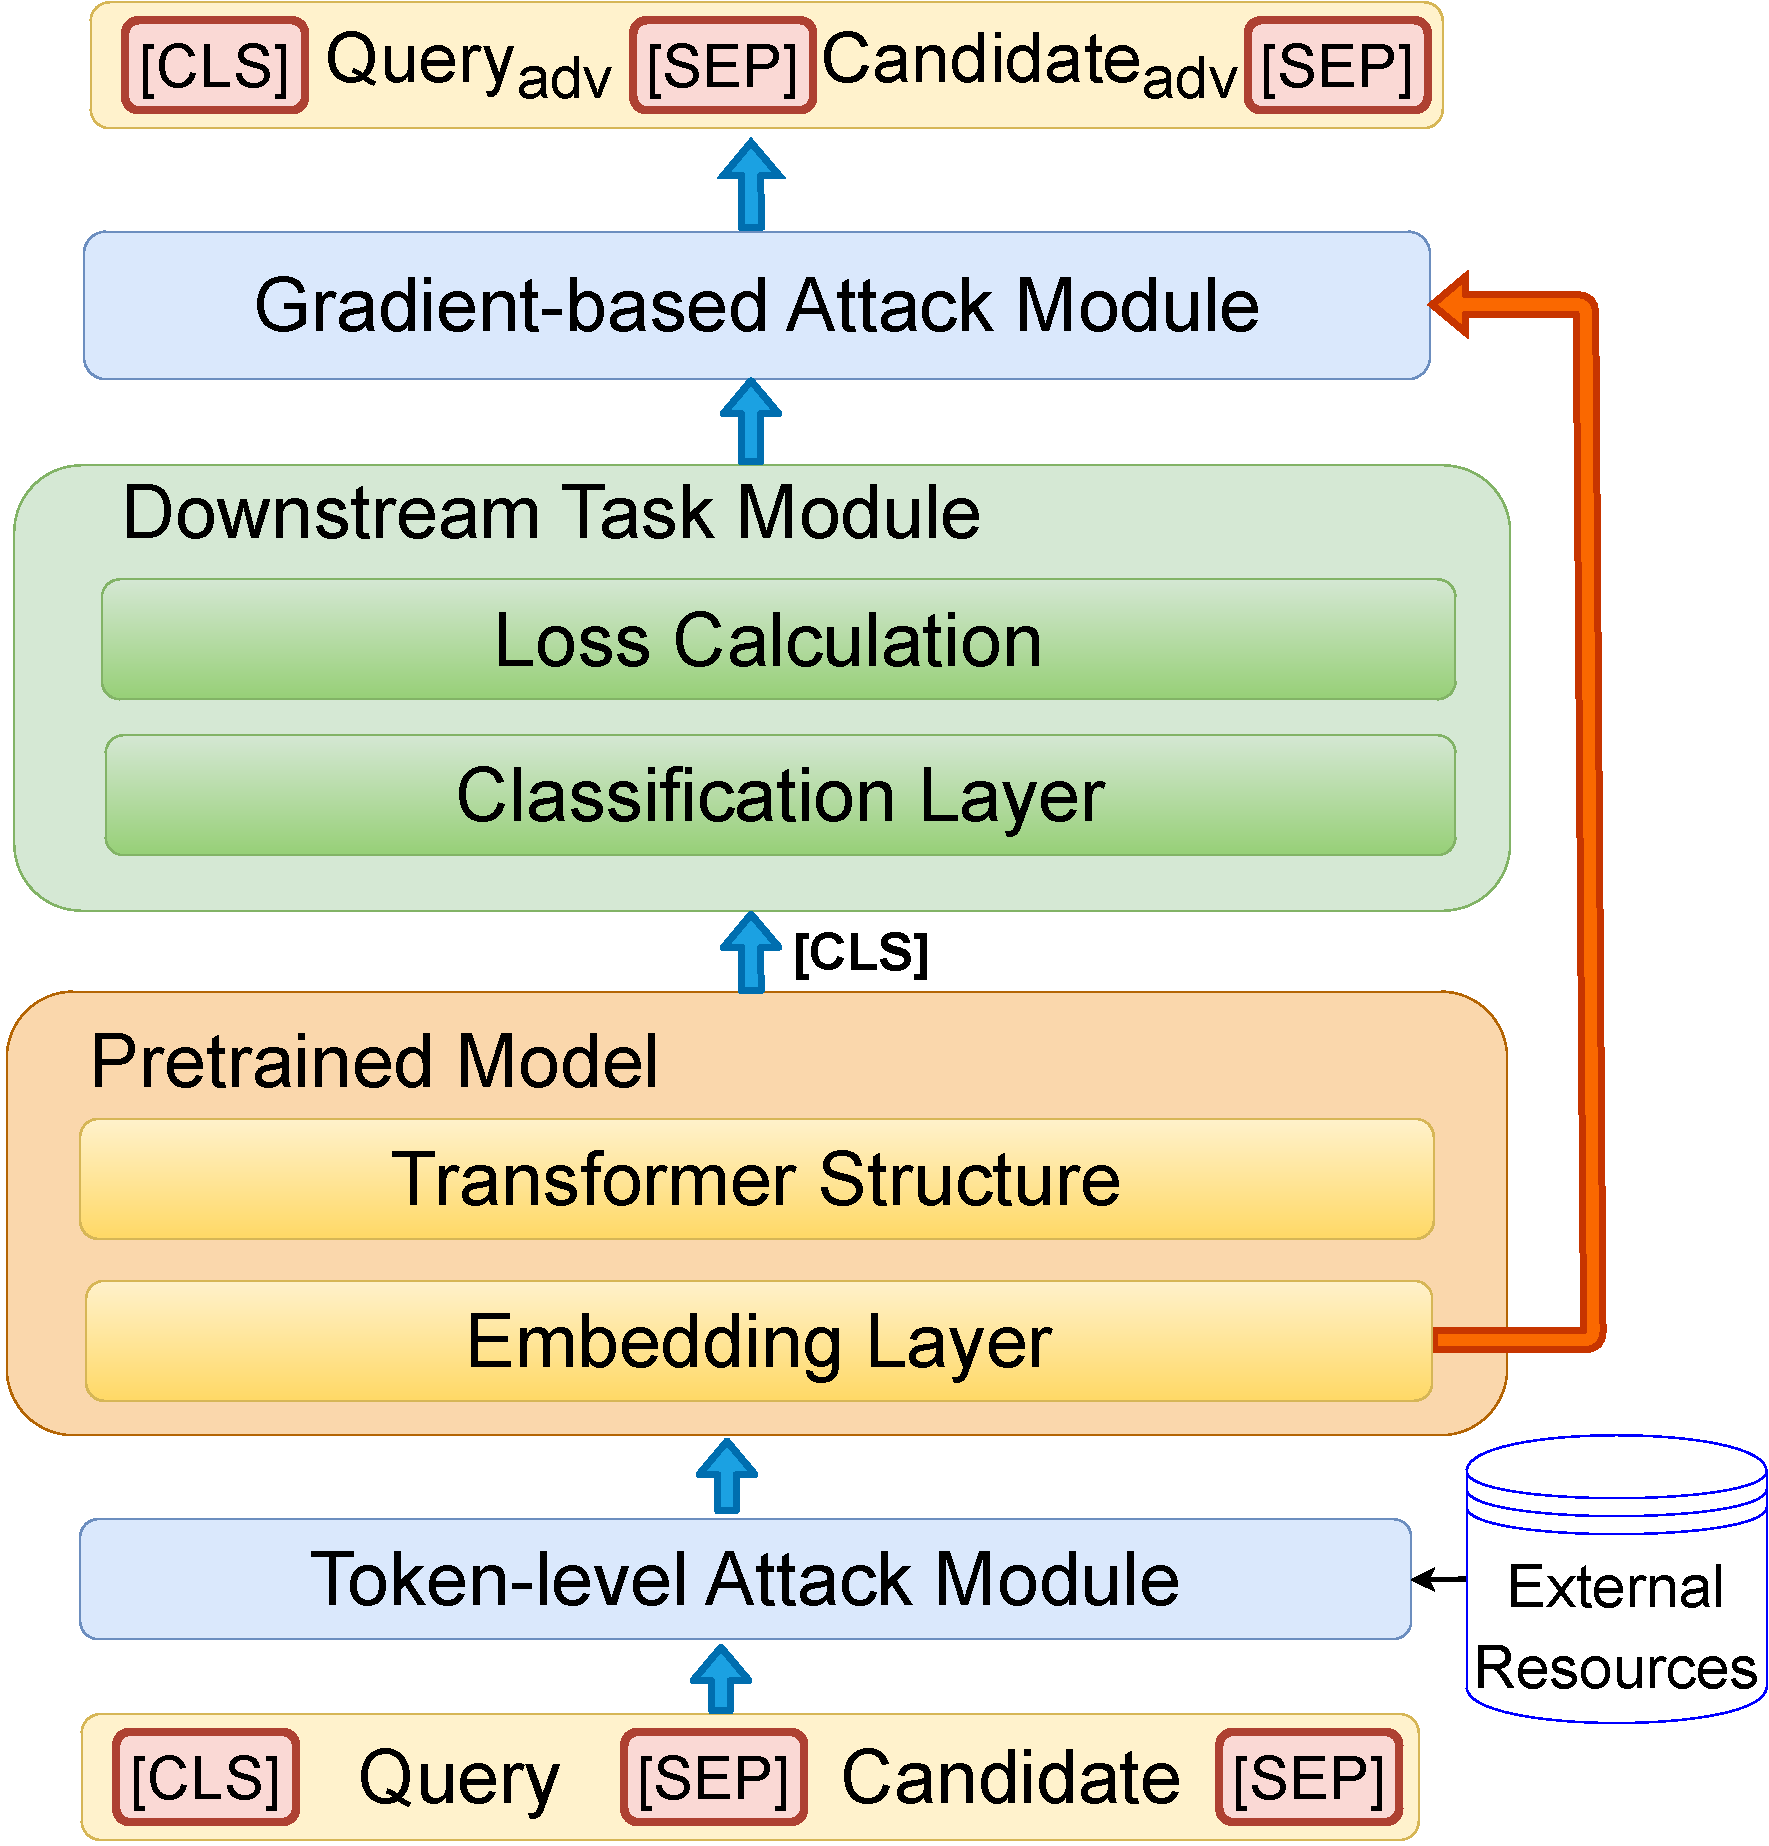
\includegraphics[width=0.5\columnwidth]{fig/fig3-2.pdf}
    \caption{对抗样本生成方法}
    \label{fig3-2}
\end{figure}

\textbf{词显著性排序} 我们的词级攻击方法希望替换句子中对于模型重要的词汇,产生对模型较大的扰动,以达到在训练中提高模型语义提取能力和稳定性的效果。
我们利用词显著性来定义词汇的重要程度,每个词$x_i$的词显著性分数$I_{x_i}$计算如下:

\begin{equation}
    I_{x_i} = Loss(F(Input_{\not {x_i}}), y) - Loss(F(Input), y)
\end{equation}

其中,$Input_{\not {x_i}}$表示将输入序列中的词$x_i$进行遮蔽。
我们分别将序列中的每个词$x_i$逐个遮蔽,观察其对损失loss的影响。
如果该词对于句子的语义信息非常关键,将其遮蔽后,损失loss必然会有明显提升,反之loss则提升不明显。
我们以这样的方式作为词重要性的排序标准,对序列中的词重要性进行排序,并留下前N\%用于同义词替换。


\textbf{同义词替换攻击} 对于每个需要替换的重要词$x_i$,我们需要选择合适的同义词进行替换,如果替换不慎,可能导致语义偏移,语法错误,甚至与原句语义完全相反。
首先,我们利用外部知识库WordNet\cite{miller1995wordnet}为$x_i$获取其同义词列表$L$。
接着,利用词性标注POS过滤$L$中词性与原词$x_i$不同的的候选单词,这一步是为了保证替换的同义词与原词词性相同,尽可能保证其语法的准确性。
此外,我们引入了反拟合嵌入空间(Counter-fitting embedding space)作为


\subsection{自适应对抗训练方法}









l



% 单词、词块和短语等语言结构在答案选择过程中往往起到至关重要的作用。
% BERT能够有效的学习到词级的上下文语义表示,但是其无法在不同颗粒度的语言结构之间实现表示学习。
% 本章在BERT的基础上,对其输出进行不同粒度的n元语法卷积编码,借以获取句子中词块、短语等语义信息,
% 继而捕获多种粒度间的交互信息,使问题与答案之间的语义交互更加充分。
% 基于BERT的多粒度交互式推理模型(MIIN)如图~\ref{fig3-1}~左侧部分所示。

% \subsection{基于BERT的预训练编码}

% 给定问句$Q=\{q_1,\ldots,q_i,\ldots,q_n\}$以及答案段落$P=\{p_1,\ldots,p_j,\ldots,p_m\}$。
% 其中,n和m分别为其文本长度,$q_i$与$p_j$分别是问句的第i个单词和答案中第j个单词。
% 本章将问句Q和答案段落P构造成$S=[[CLS],Q,[SEP],P,[SEP]]$。
% 其中,$[CLS]$是分类标志符,$[SEP]$是用以区分输入中多个句子的分句符号。
% BERT将$S$的特征表示输入多层双向Transformer\cite{vaswani2017attention}构成的编码器中,
% 从而得到问题$Q$和候选答案$P$的联合编码表示T:$T=\{T_{[CLS]},T_{[Q]},T_{[SEP]},T_{[P]},T_{[SEP]}\}$。
% 值得说明的是,Transformer含有的多头自注意力机制,能够忽略词间距计算句子中所有词对之间的依赖关系。
% 因此,联合编码表示$T$中的分布特征已经得到了初步的注意力加权。此时,加权过程仅仅依赖词(Token)级的语义信息。

% \begin{figure}[!h]
    \centering
      \includegraphics[scale=1]{figure/fig3-1.pdf}
    \caption{基于BERT的多粒度交互编码模型架构}
    \label{fig3-1}
\end{figure}

% \subsection{多粒度卷积层}

% 本章使用卷积神经网络(CNN)对BERT输出的上下文词向量进行不同粒度的编码,
% 即分别对$T_{[Q]}=\{T_{[q_1]},T_{[q_2]},\ldots,T_{[q_n]}\}$以及对应的
% $T_{[P]}=\{T_{[p_1]},T_{[p_2]},\ldots,T_{[p_m]}\}$进行不同卷积核大小的卷积操作,
% 得到其对应的隐状态表示。编码过程如下所示:
% \begin{equation}
%     h_Q^k = CNN(T_{[Q]})
% \end{equation}
% \begin{equation}
%     h_P^k = CNN(T_{[P]})
% \end{equation}
% 其中,$h_Q^k$与$h_P^k$分别是对$T_{[Q]}$和$T_{[P]}$的不同粒度编码表示,
% $k$表示卷积核的大小为$k\times d$。
% 本章采用三个尺度的卷积核($k=\{1,\ 2,\ 3\}$),对应于三类$n$元语法(Unigram,Bigram和Trigram)。
% 从语法特征看,这三种粒度的卷积能够覆盖绝大部分词块、短语等情况,形成其独立的语义表示,有助于模型获取更加丰富的语义信息。

% \subsection{多粒度交互计算}

% 本章将问句与候选答案的多粒度编码表示输入到交互单元$\eta_k$,
% 获取k-gram粒度的交互特征向量$z^k$,$\eta_k$模块具体计算过程如下:
% \begin{equation}
%     e^k=H(h_Q^k,h_P^k)
% \end{equation}
% 其中,高阶交互函数$H$将$h_Q^k$与$h_P^k$都拓展成维度为$\mathbb{R}^{(n-k+1)\times(m-k+1)\times d}$的矩阵,
% 并将其对应位置的元素数值相乘,得到交互矩阵$e^k\in\mathbb{R}^{(n-k+1)\times(m-k+1)\times d}$。

% 其次,采用多层卷积操作从交互矩阵$e^k$提取特征,多层之间参数不共享,
% 并通过最大池化层,从卷积结果中过滤出强交互信号,具体交互计算如下:
% \begin{equation}
%     \widetilde{c_i^k}=ReLU(CNN(c_{i-1}^k))
% \end{equation}
% \begin{equation}
%     c_i^k=MaxPool(\widetilde{c_i^k})
% \end{equation}
% 其中,修正的线性单元(Rectified Linear Unit,简称ReLU)\cite{nair2010rectified}相比于传统的激活函数(如sigmoid\cite{han1995influence}),
% 能够有效的避免梯度爆炸问题。$\widetilde{c_i^k}$是对交互矩阵$e^k$第$i$次卷积的结果,
% $c_i^k$是$\widetilde{c_i^k}$经过最大池化的结果($c_0^k=e^k$)。

% 最后,本章将提取到的特征矩阵$c^k$展开得到特征向量,
% 并将其输入全连接网络(Fully Connected Network,简称FC),
% 对拼接的多粒度特征向量进行推理计算得到最终高度聚合的交互特征向量$z^k$,具体过程如下:
% \begin{equation}
%     z^k=W_z^k(flatten(c^k))+b_z^k
% \end{equation}
% 其中,$W_z^k$和$b_z^k$是可训练参数,函数$flatten()$用以将交互矩阵$c^k$按照维度展开拼接为1维向量表示,特征$z^k\in\mathbb{R}^{1\times d}$。

% \subsection{答案相关性预测}

% 输出层将不同粒度的交互特征向量$z^k=\{z^1,z^2,z^3\}$与BERT分类特征向量$T_{[CLS]}$拼接得到综合性交互表示$o\in\mathbb{R}^{4\times d}$,
% 并将其输入到全连接网络中,并计算问句与答案段落的相关性分数。
% 全连接网络在反向传播的过程中,不断根据预测分数与实际结果之间的差异更新其参数值,以此自动察觉不同粒度信息的权重差异。
% 具体过程如下:
% \begin{equation}
%     o=[z^1;z^2;z^3;T_{[CLS]}]
% \end{equation}
% \begin{equation}
%     r=W_oo+b_o
% \end{equation}
% 其中,$W_o$与$b_o$为可训练参数,感知机最终输出的标量$r$即为最终相关性得分,分数高低与相关性成正比。

% \subsection{损失函数及子句损失策略}

% 本章采用Pairwise方法训练与学习答案选择任务,旨在使正样本与问题相关性得分明显高于负样本(正样本表示与问题相关的答案段落,负样本表示与问题不相关或者相关性较低的答案段落)。
% 具体而言,对于一个问题Q,Pairwise方法构造正负样本对$(Q,P^+)$与$(Q,P^-)$,并通过合页损失函数进行学习。
% 其中,$P^+$为正样本,$P^-$为负样本(若问题$Q$的正样本有$n$个,负样本有$m$个,则共有$n\ast m$个Pairwise正负样本对),正负样本答案段落合页损失计算如下:
% \begin{equation}
%     \mathcal{L}(P)=max(0,\varepsilon+r_{P^-}-r_{P^+})
% \end{equation}
% 其中,$r_{P^+}$和$r_{P^-}$分别是正负样本的相关性分数,$\varepsilon$是正负样本分数差值的阈值,函数$max()$表示从给定参数中选取最大值。

% 此外,本章在损失函数中加入子句损失,用于提升答案段落中相关程度较高的子句在答案选择过程中的作用。
% 如图~\ref{fig3-1}~所示,模型在判别答案整体与问题相关性的同时,对所有子句相关性作出预测,
% 把排名靠前的几个子句的损失添加到最终损失中,以提升关键子句的权重。
% 其中,子句与问题之间的相关性标签取决于其所属答案段落的标签。
% 若正样本$P^+=(s^{1+},\ldots,s^{i+},\ldots)$,负样本$P^-=(s^{1-},\ldots,s^{j-},\ldots)$,
% 其中$s^{i+}$表示正样本答案段落中第$i$句文本,$s^{j-}$表示负样本中第$j$句文本。
% 正负样本子句合页损失计算过程分别如下:
% \begin{equation}
%     \mathcal{L}(s^{i+})=max(0,\varepsilon+r_{s^{i+}}^--r_{s^{i+}}^+)
% \end{equation}
% \begin{equation}
%     \mathcal{L}(s^{j-})=max(0,\varepsilon+r_{s^{j-}}^+-r_{s^{j-}}^-)
% \end{equation}
% 其中,$r_{s^{i+}}^+$与$r_{s^{i+}}^-$分别为正样本中第$i$个子句与问题相关性的二分类正向分数与负向分数,
% $r_{s^{j-}}^+$与$r_{s^{j-}}^-$分别为负样本中第$j$个子句与问题相关性的二分类正负向分数。
% 通过设置超参数$sent=N$,分别从正负样本中提取与问题相关性最高的$N$个子句计算损失,
% 用这些子句损失的平均值作为该正负样本对的子句总损失。
% 总体损失则等于合页损失与子句损失的“零和”折损,计算如下:
% \begin{equation}
%     \mathcal{L}_N(s)=mean(\sum_{i}^{N}\mathcal{L}(s^{i+})+\sum_{j}^{N}\mathcal{L}(s^{j-}))
% \end{equation}
% \begin{equation}
%     \mathcal{L}=
%     \begin{cases}
%         \mathcal{L}(P), \ \ &\mathcal{L}_N(s)=0\\
%         \mathcal{L}(P)\mathcal{L}_N(s),\ \ &\mathcal{L}_N(s)>0
%     \end{cases}
% \end{equation}
% 其中,$\mathcal{L}(s^{i+})$和$\mathcal{L}(s^{j-})$分别为正负样本子句合页损失,$\mathcal{L}_N(s)$表示子句总损失,$\mathcal{L}(P)$表示正负样本答案段落合页损失,$\mathcal{L}$表示模型的总损失。

\section{实验及结果分析}

\subsection{数据集、评价方法与超参设置}
本章在WPQA数据集上进行实验,数据集的详细介绍见~\ref{2.2 语料资源概述}~小节。
实验采用平均化精度均值MAP和
平均化倒数排序MRR评价模型的排序能力,具体介绍见~\ref{2.3 性能评价指标}~小节。
本章的基线模型为BERT-base模型(12-layer, 768-hidden, 12-heads),总参数量约为110M。
输入模型的问题与答案的最大长度限制分别为40和400。
交互层使用2层卷积池化网络提取特征,卷积与最大池内核大小均为$2\times2$。
模型在训练阶段batch\_size设置为10,优化函数的学习率(learning\_rate)设置为3e-6,
优化函数中的epsilon\cite{rutherford2002lecture}设置为1e-8。子句优化策略中子句数量sent设置为2,子句最大长度限制为55。
合页损失阈值$\varepsilon$设置为1。

\subsection{前沿方法介绍}

为了验证本章所提方法的有效性,本章在WPQA数据集上与现有方法进行比较,并对其结果进行分析。
除了经典的统计模型BM25\cite{robertson1994some}和
TF-IDF(Term frequency–inverse document frequency,简称TF-IDF)\cite{ramos2003using}以外,
本章还与如下基于深度学习的前沿方法进行了比对:
\begin{itemize}
    \item \textbf{Att-BiLSTM}(Tan et al., 2016)\cite{tan2016improved}
    将注意力机制与BiLSTM (Bi-directional Long Short-Term Memory,简称BiLSTM)结合,
    使模型学习到的答案向量包含更多与问题相关的信息。
    \item \textbf{AP-BiLSTM}(Santos et al., 2016)\cite{santos2016attentive}
    在传统BiLSTM答案选择模型基础上,加入注意力层与多样化的池化层,使用行最大池与列最大池
    分别从问题与答案的交互矩阵中提取交互特征,从而使得问题特征向量中包含答案信息,答案特征向量中包含问题信息。
    \item \textbf{LW-BiLSTM}(Rücklé et al., 2017)\cite{ruckle2017representation}
    与其他基于注意力的模型相反,该方法不依赖于问题与答案的相关性,假设问题与候选答案相对独立,
    使用BiLSTM模块学习答案中单词的权重。
    \item \textbf{CA-Wang}(Wang et al., 2016)\cite{parikh2016decomposable}
    首次将Parikh等提出的Compare-Aggregate框架应用到匹配任务中,分析了多种Compare方法对模型的影响。
    \item \textbf{COALA}(Rücklé et al., 2019)\cite{ruckle2019coala}
    仅关注答案对问题的影响,使用最大池以代替注意力机制和传统的神经网络聚合层从相似度矩阵中提取问题相关特征,并使用平均化运算操作得到最终结果。
    \item \textbf{MICRON}(Han et al., 2019)\cite{han2019micron}
    使用多种n-gram卷积对问题和答案分别进行上下文编码,将其不同粒度的编码结果交叉交互,
    利用多粒度交互从问题与答案文本中提取相关信息。
    \item \textbf{BERT-PR}(Xu et al., 2019)\cite{xu2019passage}
    将预训练模型BERT应用到段落级答案选择任务中,
    同时考虑答案段落在缺少标注信息情况下的场景,使用BM25、TF-IDF等方法的投票结果作为答案段落的标签信息。
    \item \textbf{BERTlets}(Mass et al., 2019)\cite{mass2019study}
    使用BERT处理段落级答案选择任务,并通过实验分析了不同学习方式(Pointwise与Pairwise)
    以及不同文本长度限制对模型的影响。
\end{itemize}

\subsection{对比实验及分析}

表~\ref{table3-2}~列出了上述方法和本章所提方法(BERT-MIIN)在WPQA数据集上的性能。
结果显示,BERT-MIIN的MAP值和MRR值均达到最高。
经典的统计模型BM25和TF-IDF依靠特征工程的方法处理句间关系,缺乏语义理解能力,无法有效处理问题与答案之间的语义关系。
Att-BiLSTM等传统神经网络模型受到数据集大小的限制,难以充分学习到句子的语义信息,在文本较长的答案选择任务中表现不佳。
COALA模型和MICRON模型部分采用算术运算的方式代替神经网络进行交互与聚合,大大减少可训练参数量,
从而通过较少的训练数据即可取得较优效果,在一定程度上缓解了数据量限制的问题。
预训练语言模型BERT通过自监督方式在海量语料的基础上进行训练,其词向量包含丰富的上下文信息,
从而使得BERT-PR及BERTlets模型性能大幅上升。
但是,BERT-PR与BERTlets仅使用BERT的分类特征作为结果的唯一依据,且并未考虑多粒度的语义信息,从而性能低于BERT-MIIN。

\begin{table}
    \caption{模型性能对比}
    \centering
    \newcommand{\tabincell}[2]{\begin{tabular}{@{}#1@{}}#2\end{tabular}}
    \begin{tabular}{l|c|c}
    \toprule[0.7pt]
    \textbf{模型\qquad\qquad\qquad\qquad\ } & \textbf{\enspace MAP (\%)\enspace} & \textbf{\enspace MRR (\%)\enspace  } \\
    \midrule[0.7pt]

    BM25 & 53.73 & 62.58 \\
    TF-IDF & 39.92 & 46.38 \\
    \midrule[0.4pt]
    Att-BiLSTM & 47.04 & 54.36 \\
    AP-BiLSTM & 46.98 & 55.20 \\
    LW-BiLSTM & 47.56 & 54.33 \\
    CA-Wang & 48.71 & 56.11 \\
    COALA & 60.58 & 69.40 \\
    MICRON & 63.00 & 71.03 \\
    BERT-PR & 73.55 & 80.87 \\
    BERTlets & 73.60 & 81.00 \\
    \midrule[0.4pt]
    BERT(baseline) & 73.70 & 81.02 \\
    BERT-IIN & 74.02 & 81.33 \\
    BERT-MIIN & 74.84 & 82.04 \\
    \textbf{BERT-MIIN$_{sent2}$} & \textbf{75.20} & \textbf{82.21} \\
    \bottomrule[0.7pt]
    \end{tabular}
    \label{table3-2}
\end{table}

值得注意的是,BERT-IIN模型对词向量进行2-grams卷积编码(非多粒度),
以此获取问题与答案段落的局部上下文信息进行交互,其性能相较于基线有所提升。
BERT-MIIN使用多种卷积对词向量进行多粒度编码,获取到不同粒度的局部上下文信息,
并分别进行句间交互,使得问题与答案之间的交互更加充分。
由表~\ref{table3-2}~可见,BERT-MIIN的MAP和MRR指标明显高于仅采用单一粒度卷积交互的BERT-IIN,
且相较于基线分别提升了1.14\%和1.02\%。
BERT-MIIN$_{sent2}$在BERT-MIIN基础上加入了子句损失策略,
对答案段落中与问题最相关的两个子句计算损失,这有助于神经网络模型敏感地感知关键的关联语句,
并避免冗余信息对关联性判断的误导,使得MAP和MRR的性能值得以进一步提升。



\subsection{显著性分析}

实验使用显著性检验确保实验结果非偶然性,即分别计算BERT-MIIN和BERT-MIIN$_{sent2}$
对比BERT在WPQA数据集上MAP指标和MRR指标的P-value值。
P-value小于0.05表示结果存在显著差异,否则差异不显著。
由表~\ref{table3-3}~可见,本章提出的方法在统计上存在显著提升。

\begin{table}[h]
    \caption{显著性分析结果}
    \centering
    \newcommand{\tabincell}[2]{\begin{tabular}{@{}#1@{}}#2\end{tabular}}
    \begin{tabular}{l|c|c}
    \toprule[0.7pt]
    & \enspace \textbf{BERT-MIIN} \enspace& \enspace \textbf{BERT-MIIN$_{sent2}$} \enspace\\
    \midrule[0.7pt]

    MAP\qquad\quad & 0.030 & 0.018 \\
    MRR & 0.047 & 0.038 \\

    \bottomrule[0.7pt]
    \end{tabular}
    \label{table3-3}
\end{table}

\subsection{子句损失策略的性能分析}

本章使用BERT(与答案段落排序共享参数)对子句进行相关程度排序,子句的最大长度限制为55。
超参数$sent=N$表示取与答案段落中问题最相关的前$N$个子句计算损失,图~\ref{fig3-2}~通过实验分析sent取值对模型性能的影响。

\begin{figure}[h]
    \centering
      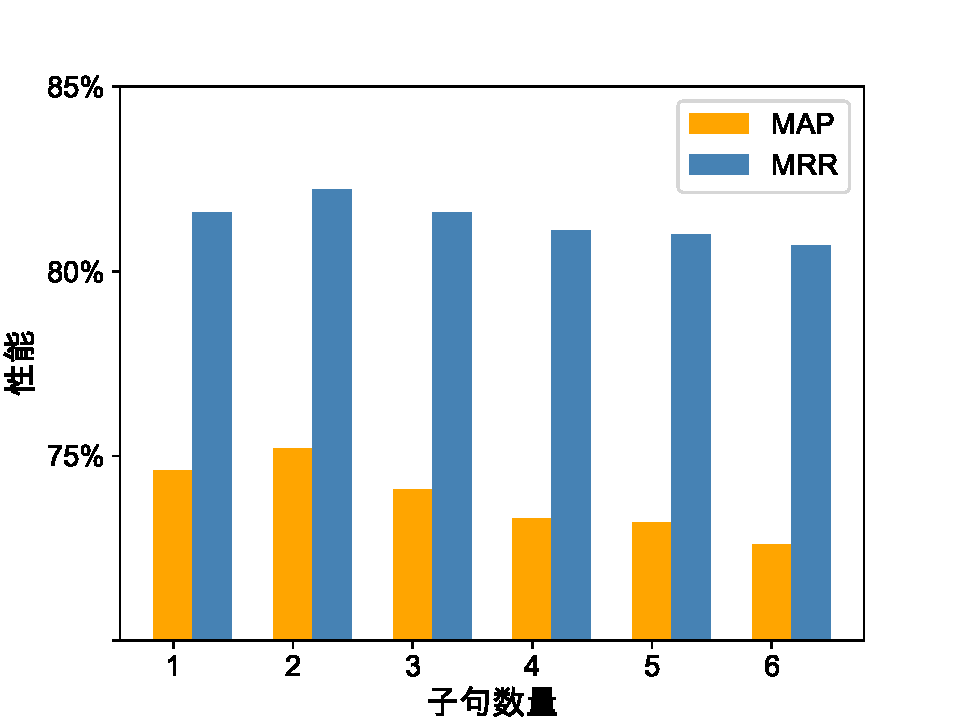
\includegraphics[scale=0.5]{figure/fig3-2.pdf}
    \caption{不同子句数量限制性能对比}
    \label{fig3-2}
\end{figure}

由图~\ref{fig3-2}~可见,当子句数量限制为2时,模型性能达到最高,
MAP和MRR值分别为75.20\%、82.21\%。实验结果表明,
部分数据的答案段落中与问题密切相关的子句往往只有1~2句。
为了验证模型对子句排序结果可信度,本章从WPQA测试集中随机取出200个问题及其候选答案段落组,
在候选答案组中取其中一个正样本(即相关答案段落)进行人工标注,与问题密切相关的子句标注为1,相关程度较低的子句标注为0。
最终共计标注1,200条子句数据,其中,与问题密切相关的子句有288条,具体信息如表~\ref{table3-4}~所示。

\begin{table}[h]
    \caption{子句测试数据统计}
    \centering
    \newcommand{\tabincell}[2]{\begin{tabular}{@{}#1@{}}#2\end{tabular}}
    \begin{tabular}{l|l|l}
    \toprule[0.7pt]
    & \;\textbf{数量} & \;\textbf{平均长度} \\
    \midrule[0.7pt]

    问题 & \;200 & \;9.78\\
    答案(子句)\quad\; & \;1,200\; & \;24.46\\
    相关答案 & \;288 & \;27.41\\

    \bottomrule[0.7pt]
    \end{tabular}
    \label{table3-4}
\end{table}

表~\ref{table3-5}~列出了在WPQA数据集上训练后,模型对人工标注数据排序的性能。
加入子句损失策略后的BERT-MIIN$_{sent2}$对子句的排序性能优于BERT和BERT-MIIN。
实验结果表明,子句损失策略不仅提升了模型在段落级答案选择任务上的性能,
同时能够对答案段落中的子句进行较为精准的相关度排序,具有一定的参考和应用价值。

\begin{table}[h]
    \caption{子句测试数据集排序性能}
    \centering
    \newcommand{\tabincell}[2]{\begin{tabular}{@{}#1@{}}#2\end{tabular}}
    \begin{tabular}{l|c|c}
    \toprule[0.7pt]
    \textbf{模型} & \enspace \textbf{MAP} \enspace& \enspace \textbf{MRR} \\
    \midrule[0.7pt]

    BERT & 82.99 & \enspace 86.02 \\
    BERT-MIIN & 84.33 & \enspace 86.53 \\
    \textbf{BERT-MIIN$_{sent2}$}\quad\; & \textbf{85.18} & \enspace \textbf{87.26} \\

    \bottomrule[0.7pt]
    \end{tabular}
    \label{table3-5}
\end{table}

\section{本章小结}

本章提出了一种多粒度交互推理模型BERT-MIIN,证明了该模型可以有效地捕获“问题与答案”之间的精细语义信息,并主动关注答案中的关键句子。
实验证明,本章提出的模型和策略在非事实性问答数据集上性能均有提升。
下一章将尝试从“问题与问题”之间语义匹配角度出发,优化问题复述识别模型的表现,
提高问答匹配技术的实际应用能力。

% 本章将进一步完善BERT-MIIN在答案选择任务中的应用,实现更深层次的语义理解与交互。
% 同时,尝试将该方法应用到其他文本匹配领域中。



